%
%
%
\section{CdTe Sensor}
\label{sec:siliconpad}
%Figure: Quantum Efficiency vs wavelength
%Photos of sensor, drawing for the circuit
The semi-conducting properties of CdTe have been studied for many decades~\cite{cdtegeneric}, 
particularly in the the context of photo-voltaic applications.
CdTe sensors are also widely used in X-ray detectors~\cite{cdtesensorsgeneric,cdtesensors2,cdtesensors3}. 
They have also been investigated for synchrotron radiation detectors in accelerator 
technology~\cite{cdtelhc}, and for three dimensional tracking for neutrino-less 
double-beta decay~\cite{Filipenko:2014zta}. In reference~\cite{cdtelhc,cdtelhc2}, poly-crystalline 
CdTe sensors have been demonstrated to have no significant degradation in
performance after irradiation of $10^{16}$ neutrons/$\mathrm{cm}^{2}$. In our previous 
studies~\cite{Anderson:2015gha,MCPShowerMaxPaper,Ronzhin201552,SiliconTiming,PixelatedMCP,Anderson:2016ygg,Anderson:2015tia} 
we have demonstrated that increasing the primary sensor signal is crucial to achieve good timing resolutions.  
CdTe sensors are available with thicknesses of $1$~mm and more, and the path-length of the charged 
shower particles in the sensor material scales up accordingly. The higher density of CdTe compared 
to Si also increases the energy loss of charged particles. 
A minimal ionizing particle will create about $50000$ electrons in 300~$\mathrm{\mu}$m 
of CdTe, compared to $30000$ electrons for a Si sensor \cite{cdtelhc2}.  The combination of these
two effects results in a larger primary signal. Furthermore, CdTe features 
a significantly higher efficiency for detecting photons in the $10-100$~keV energy range 
compared to silicon sensors. The higher atomic number of Cadmium and Tellurium, averaging 
to 48.52 for the compound bulk material, results in a higher interaction cross section for 
photons in this energy range. Secondary photons are abundant in electromagnetic showers. 
Reference~\cite{Beringer:1900zz} shows that for shower secondaries with energy over 
$1$~MeV, there are $6$ to $7$ times more photons than electrons. Therefore, an 
additional increase to the signal size resulting from the secondary photons is a promising 
possibility. The exact quantitative impact of the secondary photons will further depend 
on the depth location at which the shower is sampled and the exact material distribution 
in the vicinity of the sensor. 

%
Our measurements were conducted with a CdTe Schottky type diode purchased from 
Acrorad~\cite{acrorad}. It is $1$~$\mathrm{cm}^{2}$ in transverse size and $1$~mm thick.
It was operated at a bias voltage of $700$~V and the dark current was between $3$~nA 
and $6$~nA depending on the environmental conditions in the test-beam experimental 
zones. The sensor was placed in a box made of $0.3$~mm thick copper sheets and located
about $3$~mm away from the front face of the copper box.
A photograph of the sensor and the copper box enclosing it is shown in 
Figure~\ref{fig:CdTeSensor}.

%
\begin{figure}[htbp] 
\centering
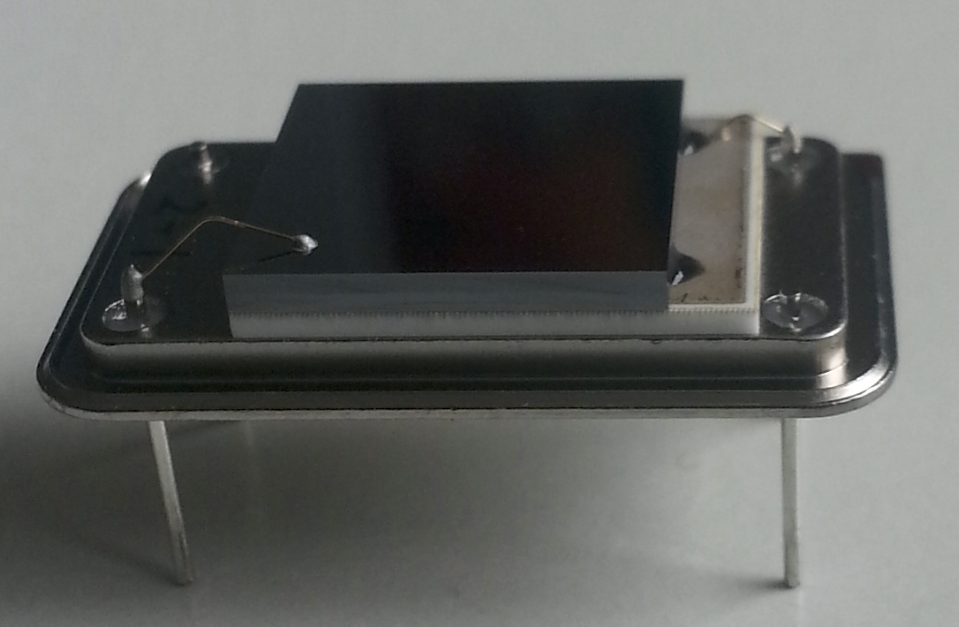
\includegraphics[width=0.44\textwidth]{figures/CdTeSensor.png} 
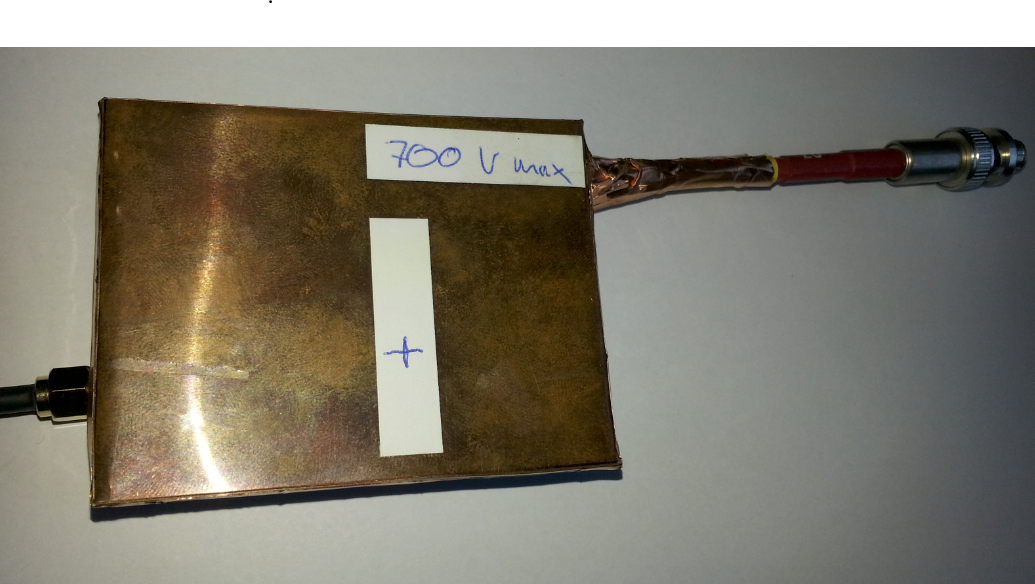
\includegraphics[width=0.55\textwidth]{figures/CdTeSensorBox.png} 
\caption{Left: CdTe sensor used for the measurements. The sensor is a Schottky type diode with a transverse size 
of $1$~$\mathrm{cm}^{2}$ and a thickness of $1$~mm. The base-plate is biased at $700$~V. 
On the front-left corner of the sensor, the wire bond connection
to the metalized top layer of the sensor can be seen. On the back-right corner,
the wire bond connection to the base-plate can be seen. 
Right: A photograph of the copper box enclosing the CdTe sensor. } 
\label{fig:CdTeSensor} 
\end{figure} 
%
The electrical circuit shown in Figure~\ref{fig:cdtecircuit} was used to connect to the sensor to the bias 
voltage with a standard high voltage cable and the readout electronics using a SMA cable with a feed 
through penetrating the copper box.

%
\begin{figure}[htbp] 
\centering
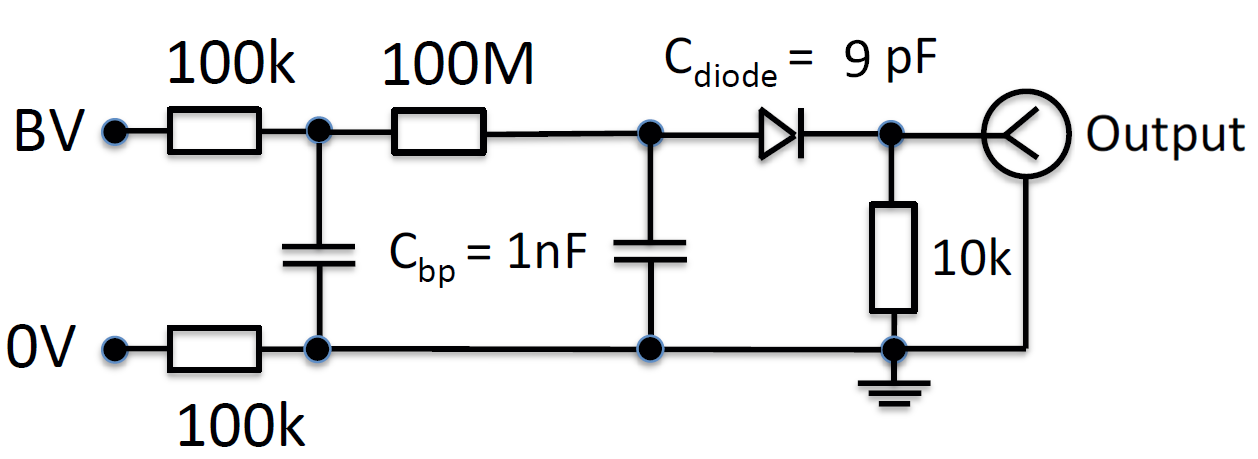
\includegraphics[width=0.49\textwidth]{figures/circuit_CdTe.png} 
\caption{Schematic diagram of the circuit used to polarize and read out the 
CdTe sensor. The circuit and the sensor are enclosed inside a copper box. }
\label{fig:cdtecircuit} 
\end{figure} 
%
